\documentclass[crop, tikz]{standalone}
\usepackage{tikz}
\usepackage{tkz-graph}

\begin{document}
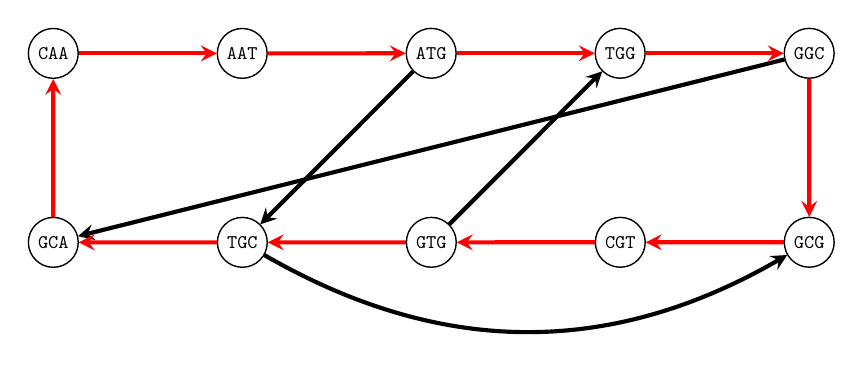
\begin{tikzpicture}[scale=0.8,every node/.style={scale=0.7},font=\tt]
	\SetUpEdge[lw         = 1.5pt,
				color      = red,
				labelcolor = white]
	\GraphInit[vstyle=Normal] 
	\SetGraphUnit{3}
	\tikzset{VertexStyle/.append  style={fill}}
	\Vertex{ATG}
	\EA(ATG){TGG}
	\EA(TGG){GGC}
	\SO(GGC){GCG}
	\WE(GCG){CGT}
	\WE(CGT){GTG}
	\WE(GTG){TGC}
	\WE(TGC){GCA}
	\NO(GCA){CAA}
	\EA(CAA){AAT}
	\tikzset{EdgeStyle/.style={-stealth, color=black}}
	\Edge(ATG)(TGC)
	\Edge(GTG)(TGG)
	\Edge(GGC)(GCA)
	\tikzset{EdgeStyle/.style={-stealth, color=black, bend right}}
	\Edge(TGC)(GCG)
	\tikzset{EdgeStyle/.style={-stealth}}
	\Edge(ATG)(TGG)
	\Edge(TGG)(GGC)
	\Edge(GGC)(GCG)
	\Edge(GCG)(CGT)
	\Edge(CGT)(GTG)
	\Edge(GTG)(TGC)
	\Edge(TGC)(GCA)
	\Edge(GCA)(CAA)
	\Edge(CAA)(AAT)
	\Edge(AAT)(ATG)
\end{tikzpicture}
\end{document}
